% presentation
\documentclass{beamer}

\usetheme{Warsaw}

% rus lang
\usepackage[main=russian,english]{babel}

% insert images
\usepackage{wrapfig}

% declare operator
\DeclareMathOperator*{\argmin}{argmin} % thin space, limits underneath in displays
\newcommand{\at}[2][]{#1|_{#2}}

% alrorithm
\usepackage{algorithm2e}
\usepackage{algorithm}
\usepackage{algpseudocode}
% \usepackage{algorithmic}

\title[Восстановление регрессии]{Лекция 2. Восстановление регрессии}
\subtitle{Основы интеллектуального анализа данных}
\author{Полузёров Т. Д.}
\institute{БГУ ФПМИ}
\date{}

\begin{document}
	
	\begin{frame}
		\titlepage
	\end{frame}
	
	
	\begin{center}
		\frametitle{Структура лекции}
		\tableofcontents	
	\end{center}
	
	
	\section{Постановка задачи}
	
	
	\begin{frame}
		\frametitle{Постановка задачи регрессии}
		Пусть имеется выборка $(X, y)_{i=1}^{\ell}$, где $X = (x_i)_{i=1}^{\ell} \subseteq \mathbb{X} = \mathbb{R}^{\ell \times n}$ - матрица признаков, $y = (y_i)_{i=1}^{\ell}\subseteq \mathbb{Y} = \mathbb{R}^{\ell}$ - вектор целевых значений.
		
		Между $\mathbb{Y}$ и $\mathbb{X}$ существует некоторая неизвестная зависимость $y^{*}: \mathbb{X} \to \mathbb{Y}$
		
		\vspace{5pt}
		
		Задача регрессии состоит в том, чтобы по имеющимся данным $(X, y)$ с помощью некоторой функции $f(x, \theta), \theta \in \Theta$ приблизить $y^{*}$ \textbf{на всем множестве} $\mathbb{X}$.
		
		\centering
		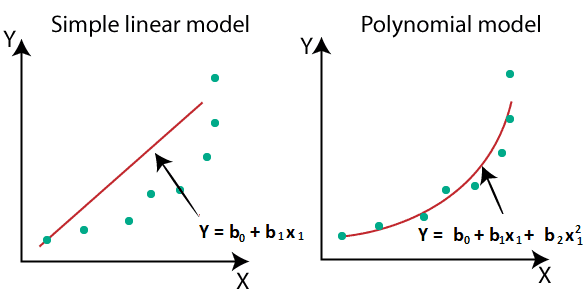
\includegraphics[width=0.7\textwidth]{img/regr_ex.png}
	\end{frame}
	
	
	\begin{frame}
		\frametitle{Метод наименьших квадратов}
		Для решения такого рода задач применяется \textbf{метод наименьших квадратов} (МНК):
		
		$$
		Q(\theta, X) = \sum_{i=1}^{\ell} (f(x_i, \theta) - y_i)^{2} \to \min_{\theta}
		$$
		В случае дифференцируемости $f$, решение находится из уравнения:
		$$
		\frac{\partial Q}{\partial \theta} = 2 \sum_{i=1}^{\ell} (f(x_i, \theta) - y_i) \frac{\partial f}{\partial \theta} = 0
		$$
		
	\end{frame}

	
	\begin{frame}
		\frametitle{Линейная регрессия}
		
		Частный случай, когда $f(x, \theta)$ линейна по своим параметрам - \textbf{линейная регрессия}
		
		$$
		a(x) = \omega_0 + \sum_{j=1}^{n} \omega_j x_j = 
		\omega_0 + \langle \omega, x\rangle 
		$$
		Определяется вектором коэффициентов $\omega = (\omega_1, ..., \omega_n) \in \mathbb{R}^{n}$ и свободным членом $\omega_0 \in \mathbb{R}$
		
		\vspace{15pt}
		
		Для упрощения формул добавим к признаковому описанию объектов признак равный единице $x := (1, x_1, ..., x_n), \omega=(\omega_0, \omega_1, ..., \omega_{n})$
		
		$$
		a(x) = \langle \omega, x \rangle
		$$
	\end{frame}	


	\begin{frame}
		\frametitle{МНК в случае линейной модели}
		
		\begin{itemize}
			\item Модель регрессии - линейная, $a(x) = \langle \omega, x \rangle$
			\item Функция потерь - квадратичная, $\mathcal{L}(a, x_i) = (a(x_i) - y_i)^{2}$
			\item Метод обучения - минимизация среднего риска, 
			$Q(\omega) = \sum_{i=1}^{\ell} (a(x_i, \omega) - y_i)^{2} \to \min\limits_{\omega}$
			%\item Проверка по тестовой выборке $X^{'} = (x_i^{'}, y_i^{'})_{i=1}^{k}]$
		\end{itemize}
	
		\vspace{15pt}
		
		В матричном виде:
		
		$$
		Q(\omega) = \frac{1}{\ell} \|X\omega - y\|^{2} \to \min_{\omega}
		$$
	\end{frame}


	\begin{frame}
		\frametitle{Точное аналитическое решение}
		Задача имеет точное аналитическое решение:
		$$
		\omega = (X^{T} X)^{-1} X^{T}y
		$$
		
		\vspace{15pt}
		
		Недостатки аналитического решения:
		\begin{itemize}
			\item Обращение матрицы $(X^{T} X)^{-1}$: в случае плохо обусловленной матрицы веса неустойчивы и очень большие по модулю. Для вырожденной матрица - обращение невозможно.
			\item Вычислительная сложность - $O(n^{2}\ell + n^{3})$
		\end{itemize}
	\end{frame}


	\begin{frame}
		\frametitle{Численное решение}
		Наиболее простой и подходящий класс методов -- \textbf{градиентные методы оптимизации}.
		
		\vspace{5pt}
		
		\begin{wrapfigure}{r}{0.3\textwidth}
			\centering
			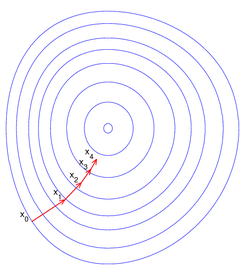
\includegraphics[width=0.35\textwidth]{img/grad.png}
		\end{wrapfigure}
		
		Общая схема:
		$$
		Q(\omega) = \frac{1}{\ell} \sum_{i=1}^{\ell} \mathcal{L}_{i}(\omega) \to \min_{\omega}
		$$
		
		$$
		\omega^{(t + 1)} = \omega^{(t)} - \alpha \cdot \nabla_{\omega} Q(\omega^{(t)})
		$$
		где $a \in \mathbb{R}$ - некоторый параметр (размер шага)
		
		\vspace{5pt}

		Градиент квадратичного функционала:
		
		$$
		\nabla_{\omega} Q = \frac{2}{\ell} X^{T}(X\omega - y)
		$$
	\end{frame}


	\section{Градиентные методы}

	
	\begin{frame}
		\frametitle{Метод градиентного спуска}
		
		\begin{algorithm}[H]
			\caption{Метод градиентного спуска}
			\SetAlgoLined
			
			\KwIn{$\alpha$ - градиентный шаг (темп обучения)}
			\KwOut{$\omega^{*}$ - оптимум функцмонала $Q(\omega)$}
			\Begin{									
				Инициализировать $\omega^{(0)}$
				
				\While{не выполнен критерий остановки}
				{
					вычислить градиент в точке
					
					$\nabla Q(\omega)\at[\big]{\omega=\omega^{(t)}} = \left( \frac{\partial Q(\omega)}{\partial \omega} \right)_{i=1}^{n}$\;
					
					\vspace{5pt}
					
					сделать шаг в сторону антиградиента
					
					$\omega^{(t + 1)} = \omega^{(t)} - \alpha \cdot \nabla_{\omega} Q(\omega^{(t)})$\;
				}
			}
			
		\end{algorithm}
	\end{frame}

	 
	\begin{frame}
		\frametitle{Идея ускорения алгоритма}
		Градиент $\nabla Q(\omega)$ представим в виде суммы градиентов:
		
		$$
		\nabla Q(\omega) = \frac{1}{\ell} \sum_{i=1}^{\ell} \nabla \mathcal{L}(\omega)
		$$
		
		Идея состоит в том, чтобы вычислять не точное значение градиента по всей выборке $X$, а оценить но некоторой подвыборке $X^{'} \subset X, |X^{'}| = k \ll \ell$ небольшого размера.
		
		$$\nabla Q(\omega) \approx \frac{1}{k} \sum_{i=1}^{k} Q(\omega)$$
		
		
	\end{frame}
	
	
	\begin{frame}
		\frametitle{Метод стохастического градиента}
		% 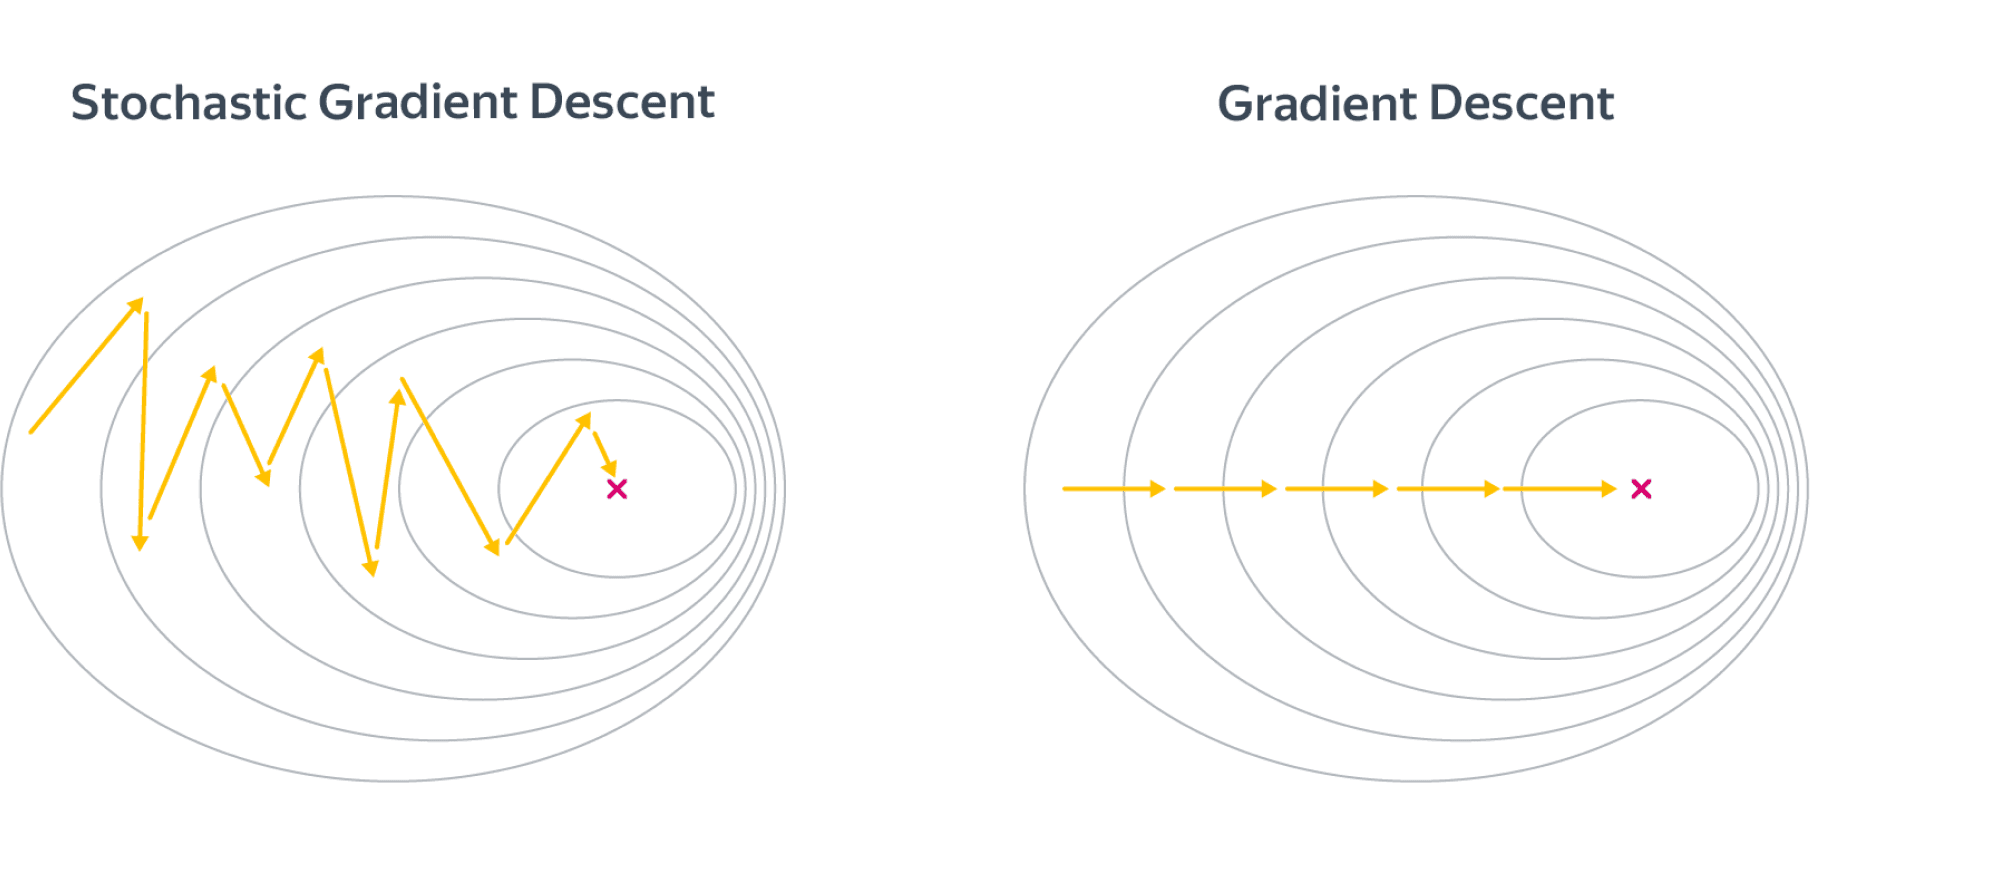
\includegraphics[width=\linewidth]{img/stoch_grad.png}
		
		\begin{algorithm}[H]
			\caption{Метод стохастического градиента}
			\SetAlgoLined
			
			\KwIn{$k$ - размер подвыборки, $\alpha$ - градиентный шаг}
			\KwOut{$\omega^{*}$ - оптимум функцмонала $Q(\omega)$}
			\Begin{
				Инициализировать $\omega^{(0)}$
				
				\While{не выполнен критерий остановки}
				{
					выбрать набор $X^{'}, |X^{'}| = k$
					
					\vspace{10pt}
					
					вычислить градиент в точке по подвыборке $X^{'}$
					
					$\nabla Q(\omega)\at[\big]{\omega=\omega^{(t)}} = \left( \frac{\partial Q(\omega)}{\partial \omega} \right)_{i=1}^{n}$\;
					
					\vspace{10pt}
					
					сделать шаг в сторону антиградиента
					
					$\omega^{(t + 1)} = \omega^{(t)} - \alpha \cdot \nabla_{\omega} Q(\omega^{(t)})$\;
				}
			}
		\end{algorithm}
	\end{frame}
	
	
	\begin{frame}
		\frametitle{Другие популярные градиентные методы}
		\begin{itemize}
			\item SAG
			\item Метод инерции (momentum)
			\item AdaGrad, RMSprop			
			\item Adam
			\
		\end{itemize}
	\end{frame}
	
	
	\section{Регуляризация}
	
	
	\begin{frame}
		\frametitle{}
		
	\end{frame}


	\section[Нелинейный случай]{Обобщение на нелинейный случай}
	
	
	\begin{frame}
		\frametitle{}
		
	\end{frame}
	
\end{document}